\chapter{TINJAUAN PUSTAKA}
\vspace{1ex}

\section*{}
Demi mendukung penelitian ini, dibutuhkan beberapa teori penunjang sebagai bahan acuan dan referensi. Dengan demikian penelitian ini menjadi lebih terarah. 
\vspace{1ex}

\section{Dasar Teori}
\vspace{1ex}

\subsection{Kardiologi}
\vspace{1ex}
Kardiologi merupakan cabang ilmu kedokteran yang mana dikhususkan mempelajari tentang gangguan jantung dan pembuluh darah. Dokter spesialis yang telah mempelajari kardiologi biasa disebut kardiolog. Akan tetapi kita harus membedakan antara kardiolog dengan ahli bedah jantung, \textit{Cardiothoracic} dan \textit{cardiovascular}, serta ahli bedah yang dapat melakukan bedah jantung menggunakan cara sternotomi. Apabila dibandingkan dengan kardiolog, ahli bedah jantung dapat melakukan operasi dengan cara membuka rongga dada kemudian melaksanakan bedah jantung, sedangkan kardiolog tidak melakukan operasi bedah, namun melakukan tes dan prosedur lain seperti angioplasti.
Kardiologi kemudian dikembangkan lagi menjadi beberapa bagian, yaitu: 
\begin{enumerate}
	\vspace{-2mm}
	\item Ekokardiografi, merupakan metode pemeriksaan jantung yang menggunakan ultrasound (gelombang suara berfrekuensi tinggi) yang dapat menangkap gambaran struktur organ jantung. Ekokardiografi biasanya dibantu dengan teknologi Doppler yang dapat mengukur kecepatan dan arah aliran darah,
	\vspace{-2mm}
	\item Elektroifisiologi Kardiak, merupakan bidang yang mempelajari sifat listrik dan kondisi penyakit jantung, serta pengobatan kelainan irama jantung (aritmia),
	\vspace{-2mm}
	\item Kardiologi Intervensional, merupakan metode perawatan jantung non-bedah yang menggunakan tabung fleksibel kecil atau kateter untuk memperbaiki struktur jantung yang rusak atau tersumbat. Beberapa prosedur yang dapat dilakukan pada jantung dengan cara kateterisasi antara lain: Angioplasti, intervensi koroner perkutan, dan valvuloplasti, 
	\vspace{-2mm}
	\item Kardiologi Nuklir, merupakan metode pemeriksaan jantung menggunakan alat nuklir yang dapat memvisualkan isotop jantung dengan menggunakan radioaktif.
	\vspace{-2mm}
\end{enumerate}
 \vspace{1ex}
 
 Dokter spesialis (kardiolog) bertugas menangani bermacam-macam gangguan terkait jantung dan sistem pembuluh darahnya. Spesifik mengenai kardiologi, jantung memiliki beberapa bagian anatomi (antara lain; atrium, ventrikel, katup) dan beberapa fitur fisiologis (antara lain; sistol, suara) yang mana telah didokumentasikan selama ratusan tahun lalu. Gangguan pada jantung dapat juga berarti mengalami sakit jantung dan sakit kardiovaskuler. Penyakit jantung dan pembuluh darah dapat mengakibatkan jumlah kematian yang cukup signifikan. Penyakit kardiovaskuler telah menyebabkan sekitar 30\%. Persentase tersebut merupakan angka yang cukup tinggi,  Karena jantung memiliki peran yang amat penting bagi tubuh yaitu memompa darah ke seluruh tubuh. Hal tersebut berarti keadaan jantung terhubung dan juga mempengaruhi seluruh keadaan tubuh. Apabila jantung memiliki masalah atau gangguan, maka tubuh juga akan terpengaruh.
 \vspace{1ex}
 
 Kardiologi telah berkembang sejak ratusan tahun lalu. Beberapa catatan kuno telah menjelaskan sedikit bahasan mengenai jantung. Pada 1241, Ibnu Sina dikomentari  oleh Ibn al-Naiis yang mana menyebut tentang sirkulasi darah saat berkomentar. Kemudian tahun 1628, dokter William Harvey dari Inggris adalah orang yang dapat menggambarkan secara tepat bagaimana sistem sirkulasi dan kandungan darah yang dipompa ke seluruh tubuh oleh jantung. Pada 1706, Profesor anatomi Raymond de Vieussens dari Prancis dapat menggambarkan struktur ruang serta pembuluh yang ada pada jantung. Beliau merupakan dokter pertama yang dapat menggambarkan bilik kiri jantung secara akurat. Kemudian pada 1733, Biarawan Stephen Hales, beliau merupakan orang pertama yang dapat mengukur tekanan darah. Perkembangan selanjutnya pada 1816, dokter René-Tnéophile-Hyacinthe Laennec berasal Prancis merupakan orang yang berhasil membuat stetoskop untuk mendiagnosis sejumlah infeksi pada rongga dada. Pada awal abad ke-19 berkembang sedikit moderen, dokter Willem Einthoven dari Belanda pada 1903 mengembangkan elektrokardiograf (ECG atau EKG) sehingga beliau berhasil meraih penghargaan Nobel Kedokteran pada 1924. Dokter Iames Bryan Herrick dari Amerika, pada 1912, beliau merupakan orang yang dapat menggambarkan gejala penyakit jantung \cite{cit:12}.
\vspace{1ex}





\subsection{ECG atau EKG}
\vspace{1ex}

Elektrokardiogram atau EKG merupakan tes yang bertujuan untuk mengukur serta merekam sinyal listrik pada jantung. Sedangkan alat yang digunakan untuk mendeteksi sinyal litrik yang dihasilkan jantung dinamakan elektrokardiograf. Elektrokardiograf dapat membaca sinyal listrik dan kemudian menggambarkan menjadi grafik yang dapat ditampilkan pada layar monitor. Metode elektrokardiogram merupakan metode yang  aman dan tidak menyakitkan karena dilakukan tanpa memberi aliran listrik secara langsung dan tidak memberi sayatan (noninvasif), serta metode ini juga tidak memakan waktu yang lama \cite{cit:13}. 

\subsection{Jenis ECG}
\vspace{1ex}

Berikut merupakan beberapa jenis tes ECG yang biasa dilakukan:
\begin{enumerate}
	\vspace{-2mm}
	\item \textit{Cardiopulmonary exercise test} (CPET)
	\vspace{1ex}
		
	CPET merupakan tes yang biasa dilakukan untuk mendeteksi penyakit jantung atau paru-paru. Saat tes CPET sedang berlangsung, pasien melakukan tes sambil berolahraga ringan dengan sepeda tegak dan bernafas melalui corong. Setiap napas pasien juga akan diukur untuk dinilai seberapa baik kinerja pada tubuh.
	Kekuatan dan kapasitas paru-paru juga diukur dan direkam terlebih dahulu sebelum berolah raga, selama berolah raga, dan sesudah berolahraga.
	Secara total, lama waktu yang diperlukan untuk tes CPET adalah sekitar 40 menit. Untuk waktu berolahraga yang dihabiskan pasien kurang lebih adalah 10 menit. Tes CPET membutuhkan upaya maksimal yang dilakukan pasien agar dapat memperoleh data yang paling bagus atau benar \cite{cit:14}.
	\vspace{-2mm}
	\item \textit{Exercise electrocardiogram (stress test)}
	\vspace{1ex}
	
	Sama seperti tes CPET, tes stress juga dilakukan pasien sambil berolahraga dengan mengayuh sepeda statis atau dengan berjalan diatas treadmill. 
	Tes Stress memiliki tujuan untuk memantau kondisi selama keadaan stres. Tes stress biasanya dilakukan setelah pasien mengalami serangan jantung, operasi jantung, dan juga saat terdeteksi mengalami penyakit arteri koroner \cite{cit:14}.
	\vspace{-2mm}
	\item \textit{Monitor Holter}
	\vspace{1ex}
	
	Holter merupakan jenis perangkat yang dapat dipakai untuk mendapat impuls listrik dari jantung yang bisa digunakan untuk memantau keadaan jantung selama 24 jam atau lebih. Elektroda ditempatkan sesuai tempat tertentu pada dada, lengan, dan kaki.
	Elektroda tersebut terhubung dengan mesin elektrokardiograf melalui kabel timah, sehingga aktivitas jantung dapat dideteksi, divisualisasikan dan kemudian dicetak untuk diinformasikan kepada dokter \cite{cit:14}.
	\vspace{-2mm}
	\item \textit{Resting}12-lead EKG
	\vspace{1ex}
	
	Resting 12-lead EKG merupakan tes yang ideal mengetahui sinyal listrik dari keadaan jantung pasien. Tes ini dilakukan saat keadaan rest atau tidak beraktivitas yang mana pasien menjalani tes ini sambil diam berbaring, setelah itu perangkat 12-lead EKG akan mengukur aktivitas kelistrikan jantung melalui 12 elektroda ysng dipasang pada dada, lengan, dan kaki pasien secara bersamaan.
	Tes ini merupakan jenis yang dapat dipakai secara rutin untuk memantau kondisi jantung sebelum gejala berkembang \cite{cit:14}.
	\vspace{-2mm}
	\item \textit{Signal-averaged electrocardiogram }(SAECG)  
	\vspace{1ex}
	
	Tes SAECG merupakan jenis dengan teknik elektrokardiografi khusus, di mana beberapa sinyal listrik dari jantung dirata-ratakan untuk menghilangkan interferensi dan mengungkapkan variasi kecil pada kompleks QRS, biasanya disebut "potensial akhir". Ini mungkin merupakan kecenderungan terhadap \textit{ventricular tachyarrhythmias} yang berpotensi berbahaya. Tes SAECG dilakukan selama kurang lebih 20 menit untuk mendeteksi adanya aritmia dalam durasi pendek \cite{cit:14}.
\end{enumerate}

\subsection{Sinyal ECG}
\begin{figure}[H]
	\begin{center}\centering
		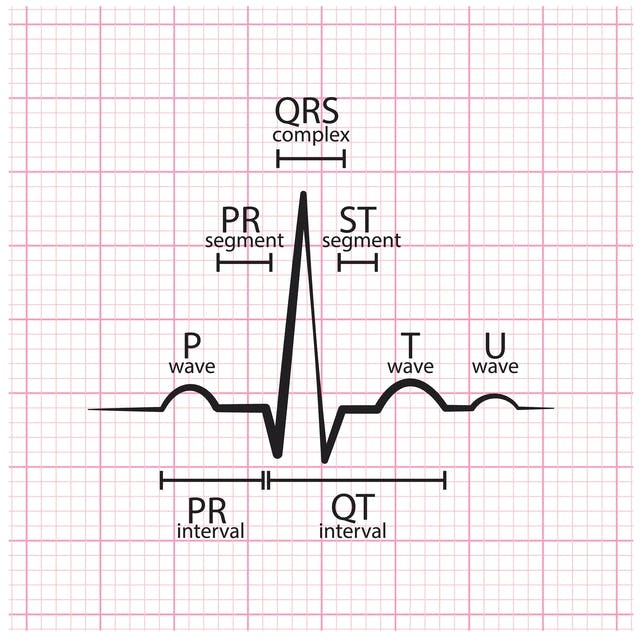
\includegraphics[scale=0.3]{img/Sinyal ecg}
		\caption{Gelombang ECG.}
		\label{fig:2.0}
	\end{center}
\end{figure}

Sinyal atau gelombang ECG merupakan gambaran atau visualisasi data dari aktivitas kelistrikan pada jantung yang telah diukur menggunakan sensor ECG. Gelombang ECG normal terdiri dari 3 bagian dasar. Yang pertama adalah gelombang P (sebelum lonjakan) yang mana menggambarkan aktivitas pada atrium yang memeras darah ke bawah menuju ventrikel. Kedua adalah QRS kompleks yang tampak seperti lonjakan menggambarkan mewakili dua ventrikel yang memeras darah ke tubuh dan paru-paru. Dan yang ketiga adalah gelombang T pada posisi terakhir mencerminkan pemulihan ventrikel saat menjadi rileks untuk menerima darah lagi\cite{cit:10}.
\vspace{1ex}


\subsection{AD8232}
\vspace{1ex}
\begin{figure}[H]
	\begin{center}\centering
		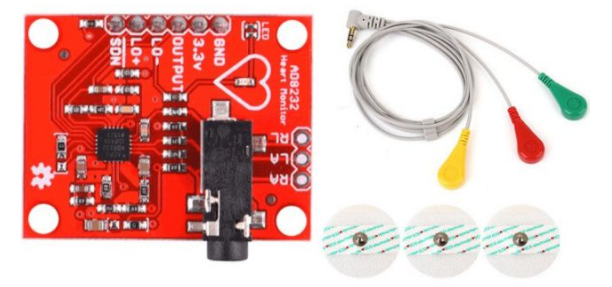
\includegraphics[scale=0.7]{img/AD8232}
		\caption{Sensor AD8232.}
		\label{fig:2.1}
	\end{center}
\end{figure}

AD8232 adalah sensor yang dapat mendeteksi sinyal terintegrasi yang bisa dipakai untuk tes pengukuran detak jantung dan aplikasi pengukuran biopotensial lainnya. AD8232 menggunakan IC pada yang terpasang pada boardnya yaitu modul SEN-12650, modul tersebut memiliki jack 3.5 female yang berfungsi untuk menancapkan kabel elektroda. AD8232 dirancang agar dapat mengekstrak, memperkuat, dan memfilter sinyal biopotensial kecil di hadapan kondisi bising, seperti suara yang dibuat oleh gerakan tubuh. Modul AD8232 memiliki sembilan pin, yaitu SDN, LO +, LO-, OUTPUT, 3.3V, GND, dan juga disediakan pin RA (Lengan Kanan), LA (Lengan Kiri), dan RL (Kaki Kanan) yang dapat dihubungkan dengan tambahan sensor AD8232 yang lain untuk membuat custom jumlah leadnya. Selain itu, modul AD8232 memiliki lampu indikator LED yang akan berkedip mengikuti irama detak jantung\cite{cit:5}.
 
\vspace{1ex}

\subsection{AD8232 \textit{Placement}}
\vspace{1ex}

Dengan modul AD8232, elektroda dihubungkan melalui jack audio. Output buffer dan filter tersedia melalui output analog yang dapat dibaca oleh input analog pada mikrokontroler. Berikut ini merupakan 2 macam penempatan electrode yang ditunjukkan pada Gambar \ref{fig:2.1.0}.
\begin{figure}[H]
	\begin{center}\centering
		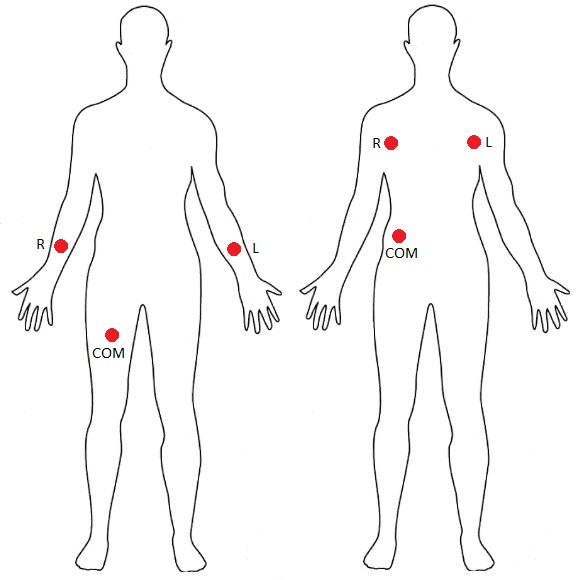
\includegraphics[scale=0.5]{img/AD8232-Electrode-Placement-1}
		\caption{Penempatan AD8232 1 (kiri), Penempatan AD8232 2 (kanan)}
		\label{fig:2.1.0}
	\end{center}
\end{figure}
Berdasarkan gambar tersebut, terdapat 2 macam penempatan electrode. Perbedaan penempatan tersebut tidak mempengaruhi data yang dihasilkan sensor sehingga pengguna bebas memilih salah satu penempatan electrode berdasarkan gambar tersebut.
Elektroda mendeteksi perubahan listrik yang terjadi saat jantung melewati proses detak jantung. Elektroda mendeteksi sinyal listrik kecil yang berada dalam kisaran beberapa ratus mikrovolt ke monitor EKG yang memproses sinyal. Pemrosesan melibatkan amplifikasi dan penyaringan dan kemudian data disediakan dalam format yang dapat digunakan untuk memperbarui tampilan dari beberapa jenis \cite{cit:22}.
\vspace{1ex}

\subsection{Modul Bluetooth HC-05}
\vspace{1ex}

Modul Bluetooth HC-05 merupakan konverter Bluetooth ke serial yang dapat digunakan untuk menghubungkan antara mikrokontroler (seperti Arduino) dengan perangkat berkemampuan Bluetooth lainnya. Pinout dan deskripsi HC-05 adalah seperti berikut:
\begin{enumerate}
	\vspace{-2mm}
	\item \textbf{KEY/En}, Pin ini digunakan untuk membawa modul Bluetooth dalam mode perintah AT. Secara default, pin ini beroperasi dalam mode data. Pin Kunci/EN harus tinggi untuk mengoperasikan Bluetooth dalam mode perintah. Di HC-05, kecepatan baud default dalam mode perintah adalah 38400bps dan 9600 dalam mode data,
	\vspace{-2mm}
	\item \textbf{VCC}, Digunakan untuk memberi daya pada modul Bluetooth. Berikan 5V / 3,3 V ke Pin ini,
	\vspace{-2mm}
	\item \textbf{GND}, Pin ground dari modul,
	\vspace{-2mm}
	\item \textbf{TXD}, Hubungkan pin ini dengan pin RXD Mikrokontroler. Pin ini mentransmisikan data Serial (sinyal nirkabel yang diterima oleh modul Bluetooth diubah oleh modul dan ditransmisikan secara serial pada pin ini),
	\vspace{-2mm}
	\item \textbf{RXD}, Hubungkan pin ini ke pin TXD Mikrokontroler. Modul Bluetooth HC-05 menerima data dari pin ini dan kemudian mentransmisikannya secara nirkabel,
	\vspace{-2mm}
	\item \textbf{State}, Ini digunakan untuk memeriksa apakah modul terhubung atau tidak. Ini bertindak sebagai indikator status.
\end{enumerate}

Modul Bluetooth HC-05 dapat digunakan dalam dua mode operasi: Mode Perintah dan Mode Data. Modus Perintah,
dalam Mode Perintah kita dapat berkomunikasi dengan modul Bluetooth melalui AT Commands untuk mengonfigurasi berbagai pengaturan dan parameter Modul. Ini termasuk informasi firmware, mengubah Baud Rate, mengubah nama modul, dll. Kita juga dapat menggunakannya untuk mengatur HC-05 sebagai master atau slave. Untuk memilih salah satu mode, kita perlu mengaktifkan Mode Perintah dan mengirimkan Perintah AT yang benar. Baud rate defaultnya adalah 38400bps dalam mode perintah .

Modus Data,
dalam mode ini modul digunakan untuk berkomunikasi dengan perangkat Bluetooth lain, yaitu transfer data terjadi dalam mode ini. Pertukaran data antar perangkat. Baud rate defaultnya adalah 9600bps dalam mode data \cite{cit:20}.

\vspace{1ex}


\subsection{Arduino Nano}
\vspace{1ex}


  \begin{table}[h]
 	\begin{tabular}{|l|l|}
 		
 		\hline
 		\multicolumn{1}{|c|}{{\color[HTML]{000000} \textbf{Spesification}}} & \multicolumn{1}{c|}{\textbf{Values}} \\ \hline
 		Microcontroller & Atmel ATmega168 for Arduino \\& Nano 2.x,  \\ 
 		& Atmer ATmega328 for Arduino \\& Nano 3.x \\ \hline
 		Operating voltage & 5 Volt \\ \hline
 		Input voltage & Optimal: 7-12 Volt \\& Min: 6 Volt\\& Max: 20 Volt \\ \hline
 		Digital I/O pins & 14 pins (D0-D13) \\ \hline
 		Analog pins & 8 pins (A0-A7) \\ \hline
 		Maximum electric current & 40 mA \\ \hline
 		Clock speed & 16 Mhz \\ \hline
 		SRAM &  1 kbyte (ATmega168) \\& and 2 kbyte (ATmega328) \\ \hline
 		EEPROM & 512 byte (Atmega168) \\& and 1 kbyte (Atmega328) \\ \hline
 		Flash memory & 32 Mbyte for Arduino Nano 3.x
 		
 		\\& 16 Mbyte for Arduino Nano 2.xz \\ \hline
 		Board size & 4,5 mm x 18 mm \\ \hline
 		Weight & 5 grams \\ \hline	
 		
 	\end{tabular}
 	\vspace{1ex}
 	\caption{Spesifikasi Arduino Nano \cite{cit:19}}
 	\label{tabel:2.0}
 \end{table}
 Perangkat Arduino yang digunakan pada penelitian ini yaitu Arduino Nano. Hal ini karena pada penelitian ini hanya memfokuskan untuk mengirimkan data sinyal dari arduino kepada dokter melalui aplikasi. Berdasarkan hal tersebut maka pada penelitian ini tidak membutuhkan banyak port untuk arduino. Perlu diketahui bahwa pada penelitian ini hanya membutuhkan 1 port analog untuk dihubungkan dengan pin output dari sensor AD8232. Arduino memiliki port ADC yang mana dapat mengkonversi sinyal analog menjadi digital. Pada Arduino Nano terdapat 8 port analog (A0-A7).  Spesifikasi dari Arduino Nano dapat dilihat pada Tabel \ref{tabel:2.0}.
 \clearpage
 

\vspace{1ex}






\section{Penelitian Terkait}
\vspace{1ex}

\subsection{\textit{IoT based Real Time ECG Monitoring System using Cypress WICED}}
\vspace{1ex}
Pada tahun 2017, Uttam U. Deshpande dan Milan A. Kulkarni mengerjakan penelitian, penelitian tersebut merancang dan menerapkan sistem pemantauan ECG berdasarkan \textit{Cypress Wireless Internet Connectivity for Embedded Devices} (WICED) dan membandingkannya dengan  Wi-Fi, Bluetooth, Zigbee dan BLE untuk membuktikan kecepatannya mengirim data yang lebih tinggi dan memiliki cakupan area yang lebih luas.\cite{cit:4}
\vspace{1ex}

\subsection{\textit{An IoT-cloud Based Wearable ECG Monitoring System for Smart Healthcare}}
\vspace{1ex}

Pada tahun 2016, Zhe Yang, Qihao Zhou, Lei Lei, Kan Zheng, dan Wei Xiang melakukan penelitian, yang mana merancang dan menerapkan sistem pemantauan EKG berdasarkan teknik IoT cloud. Penetian ini juga menggunakan Wi-Fi, Bluetooth, Zigbee dan BLE untuk mengirim data ke cloud. Cloud IoT bertanggung jawab untuk memvisualisasikan data EKG kepada pengguna dan menyimpan data untuk analisis lebih lanjut, yang diimplementasikan atas dasar tiga server, yaitu server HTTP, Server MQTT, dan server penyimpanan.\cite{cit:7}
\vspace{1ex}

